\section{Datasheet for Datasets}
\label{app:datasheet}

\paragraph{Motivation.}
OMol-Descriptors-4M was created to extend the OMol25 corpus~\citep{levine2026openmolecules2025omol25} with
post-DFT interpretive descriptors: partial charges, bond orders, QTAIM
topology, fuzzy and surface integrations, and ORCA global features (which where in OMol25) that have
historically been absent from large-scale ML-ready quantum-chemical datasets.
The dataset is intended for training descriptor-aware ML models and for
benchmarking surrogates that approximate wavefunction-derived quantities
without per-molecule DFT.
The dataset was created by the authors at the authors' home institution.
Funding sources are listed in the Acknowledgments.

\paragraph{Composition.}
Each instance is a single molecular structure with associated wavefunction-derived
descriptors. The corpus contains 3{,}986{,}738 structures (the publicly released
4M wavefunction subset of OMol25) spanning 80+
elements. Per-structure data is sharded across eight LMDB files
(Section~\ref{sec:storage}); the descriptor families are enumerated in
Section~\ref{sec:dataset}. Splits are described in Section~\ref{sec:eval}.
The corpus contains no human subjects, personally identifiable information, or
confidential data.

\paragraph{Collection Process.}
Geometries, wavefunctions, density matrices, and ORCA output files were
inherited from the OMol25 4M electronic structure release. We did not collect new DFT calculations;
all post-processing was applied to artifacts already produced by the OMol25
authors at the $\omega$B97M-V/def2-TZVPD level.

\paragraph{Preprocessing / Cleaning / Labeling.}
Wavefunctions were processed through the open \texttt{generator} pipeline
(Section~\ref{sec:pipeline}), wrapping Multiwfn~\citep{multiwfn} and
ORCA~\citep{orca5} post-analysis utilities. JSON outputs were validated and
compacted into LMDB shards keyed by relative job-folder path. Conversion is
essentially lossless (Section~\ref{sec:dataset-quality}); all raw artifacts
remain available in the OMol25 release for users wishing to reprocess.

\paragraph{Uses.}
Intended uses include training ML models that predict charges, bond orders,
or QTAIM properties; benchmarking descriptor-aware MLIPs; and serving as a
target for surrogate models that compress the full DFT-then-Multiwfn pipeline.
Inappropriate uses include drawing chemistry conclusions outside the OMol25
level of theory or extrapolating to excited-state regimes (see \S\ref{sec:limits}).

\paragraph{Distribution.}
The dataset is released on Hugging Face under a CC-BY-4.0 license, inheriting
OMol25's license terms: \url{https://huggingface.co/datasets/neuripssub2026test/OMol-Descriptors-4M}.
The \texttt{generator} pipeline is released under MIT license at
\url{https://anonymous.4open.science/r/qtaim_generator-8C0C/README.md}. No third-party IP, export controls, or fees
apply.

\paragraph{Maintenance.}
The dataset will be maintained by the authors at Lawrence Berkeley National
Laboratory. Issues, errata, and feature requests can be filed on the code
repository. Updates, including the planned merge with OMol25 energies and
forces, and additional descriptor schemes (MBIS, IBSI, CHELPG), will be
released as versioned HF records with changelogs. Older versions will
remain accessible.

\section{Compute Resources}
\label{app:compute}

Post-processing of the 4M-structure subset was carried out on
three HPC systems:

\begin{itemize}
  \item \textbf{Tuolumne} (Lawrence Livermore National Laboratory). El Capitan
    sibling system used for the highest-throughput phase of Multiwfn-driven
    QTAIM, charge, bond-order, and fuzzy-integration jobs.
    \url{https://hpc.llnl.gov/hardware/compute-platforms/tuolumne}
  \item \textbf{ALCF Crux} (Argonne Leadership Computing Facility, Argonne
    National Laboratory). AMD EPYC-based system used for additional
    descriptor generation and Parsl-managed workflow batches.
    \url{https://www.alcf.anl.gov/crux}
  \item \textbf{Lawrencium LR7, LR6 partitions} (Lawrence Berkeley National
    Laboratory High-Performance Computing). Used for ORCA conversions
    (\texttt{orca\_2mkl}), JSON-to-LMDB sharded conversion, and analytical
    notebook workloads.
    \url{https://scienceit-docs.lbl.gov/hpc/systems/lawrencium/}
\end{itemize}


\section{Held-Out Construction Logic}
\label{app:heldout}
% Detailed construction for H1--H8.

\subsection{H1 metal-ligand pair selection}
\label{app:heldout-h1}

\begin{itemize}
  \item Element-pair co-occurrence (859 TM pairs in
    \texttt{metal\_nonmetal\_pairs.csv}) is a coarse upper bound;
    selection here uses true bonds (Mayer / fuzzy bond order $\geq 0.3$)
    extracted from \texttt{bond.lmdb} via \texttt{tm\_neighbor\_lists.py}.
  \item Per-vertical bond extraction across 15 TM-bearing verticals;
    one row per (TM atom, partner atom) bond.
  \item Global pair table: \textbf{1{,}101 unique (TM, partner) bond
    pairs} across \textbf{651{,}742 TM-bonded structures} (16.35\% of
    dataset).
  \item Frequency bands (log-spaced): B1 $[1,10)$ 529 pairs;
    B2 $[10,100)$ 93; B3 $[100,1k)$ 233; B4 $[1k,10k)$ 203;
    B5 $[10k,100k)$ 43.
  \item Stratified sampling shape $(3, 2, 2, 4, 0)$,
    \texttt{numpy.random.default\_rng(seed=87)}. B5 excluded (Pt-C,
    Ti-H, etc. dominate training); B4 capped at 4 to keep realized
    holdout near 15k.
  \item Selected pairs: \emph{B1} Pt-Na, Rh-Fe, Ag-Pd; \emph{B2} Sc-Ir,
    Cd-Sb; \emph{B3} Mn-Sb, Ir-Ge; \emph{B4} Tc-Cl, Re-H, Sc-S, Hf-C.
  \item Variance: across 30 seeds with shape $(3,2,2,4,0)$, realized
    size is $15{,}227 \pm 4{,}871$. Seed 87 lands within 200 of the 15k
    target.
  \item Reproducibility:
    \texttt{qtaim\_gen/source/analysis/build\_holdout\_csvs.py}; outputs
    \texttt{h1\_metal\_ligand\_pair\_definitions.csv} and
    \texttt{h1\_metal\_ligand\_pairs.csv}.
\end{itemize}

\subsection{H6 lanthanide-ligand pair selection}
\label{app:heldout-h6}

\begin{itemize}
  \item Same construction as H1, applied to (Ln, partner) bonds via
    \texttt{tm\_neighbor\_lists.py --element\_class ln}.
  \item Five Ln-bearing verticals: \texttt{omol}, \texttt{tm\_react},
    \texttt{ml\_mo}, \texttt{electrolytes\_reactivity},
    \texttt{mo\_hydrides}.
  \item Global pair table: \textbf{453 unique (Ln, partner) bond pairs}
    across \textbf{66{,}677 Ln-bonded structures} (1.67\% of dataset).
    All 15 lanthanides represented.
  \item Frequency bands: B1=207, B2=102, B3=86, B4=58, B5=0 (max pair
    size 4{,}439). H6 effectively samples four bands.
  \item Stratified sampling shape $(3, 2, 2, 1, 0)$, \texttt{seed=190}.
    B4 toned down to 1 vs H1's 4 (Ln B4 is sparser, target $\sim$2.5k).
  \item Selected pairs: \emph{B1} Lu-Ni, Ce-La, Gd-Sb; \emph{B2} Ho-F,
    Yb-Si; \emph{B3} Dy-S, Nd-S; \emph{B4} Tm-N.
  \item Reproducibility: same build script as H1; outputs
    \texttt{h6\_lanthanide\_ligand\_pair\_definitions.csv} and
    \texttt{h6\_lanthanide\_ligand\_pairs.csv}.
\end{itemize}

\subsection{Holdout-Aware Splitting Pipeline}
\label{sec:eval-pipeline}

\begin{itemize}
  \item \textbf{Step 1 -- Pull holdouts.}
    \texttt{pull\_holdout\_records.py} reads each holdout CSV,
    materializes per-set LMDBs under \texttt{data/holdouts/<set>/}, and
    emits a \texttt{manifest\_holdout.parquet} keyed on the LMDB key
    convention
    \texttt{relpath(folder, root\_dir).replace(os.sep, "\_\_")}.
  \item \textbf{Step 2 -- Exclude.}
    \texttt{multi\_vertical.load\_exclusion\_set} re-derives LMDB keys
    from the manifest \texttt{rel\_path} column and unions
    H1/H3/H6/H7/H8 into one per-vertical exclusion set.
  \item \textbf{Step 3 -- Split.} \texttt{split\_descriptor\_lmdbs.py}
    reads \texttt{structure.lmdb}, drops excluded keys, assigns each
    remaining key to train/val/test by
    \texttt{BLAKE2b(formula\_hill) \% 10}, then partitions each of the
    8 descriptor LMDBs (\texttt{structure}, \texttt{charge},
    \texttt{qtaim}, \texttt{bond}, \texttt{fuzzy}, \texttt{other},
    \texttt{orca}, \texttt{timings}) into the assigned split.
  \item Output layout:
    \texttt{<output\_dir>/<vertical>/<split>/<descriptor>.lmdb}.
  \item HPC parallelism: \texttt{--include\_verticals X} +
    \texttt{--merge\_from DIR}, mirroring the pull pipeline.
    Per-vertical \texttt{split\_assignment.json} is the durable,
    race-free record (no global plan file).
  \item Lock-step audit: across all 8 descriptors, source row count $=$
    train $+$ val $+$ test $+$ excluded for every vertical (verified on
    \texttt{ani2x}: 215{,}642 source $=$ 168{,}783 + 17{,}417 +
    29{,}442, $n_{\mathrm{excluded}}=0$).
\end{itemize}

%\section{Per-Method Descriptor Definitions}
%\label{app:descriptors}

%\section{HPC Configuration Files}
%\label{app:hpc}
% NERSC + ALCF Parsl configs.

\section{Per-Vertical Census Table}
\label{app:t1_census}

Table~\ref{tab:t1_census} expands Sec.~\ref{sec:census} into the full
per-vertical breakdown (34 verticals plus the corpus total).
Figure~\ref{fig:descriptor_density_app} reports per-structure descriptor
density for atoms and QTAIM bond critical points.

\begin{scriptsize}
\setlength{\tabcolsep}{2.5pt}
\begin{longtable}{lrrrrrrrr}
\caption{Per-vertical census of OMol-Descriptors-4M. Counts are
corpus-level pre-split totals. \textit{Structs}: structure count.
\textit{Forms}: unique alphabetical formulas. \textit{Atoms}: atom-level
descriptor records. \textit{Charge rec.}: per-job per-method charge-scheme
records. \textit{BCPs}: QTAIM bond critical points.
\textit{Mayer / L\"owdin / Fuzzy}: per-scheme bond-order records.}
\label{tab:t1_census} \\
\toprule
Vertical & Structs & Forms & Atoms & Charge rec. & BCPs & Mayer & L\"owdin & Fuzzy \\
\midrule
\endfirsthead
\multicolumn{9}{l}{\small\textit{Table~\ref{tab:t1_census} continued from previous page}} \\
\toprule
Vertical & Structs & Forms & Atoms & Charge rec. & BCPs & Mayer & L\"owdin & Fuzzy \\
\midrule
\endhead
\midrule
\multicolumn{9}{r}{\small\textit{continued on next page}} \\
\endfoot
\bottomrule
\endlastfoot
\texttt{5A\_elytes}              &     14{,}200 &     11{,}294 &   2{,}325{,}187 &      99{,}383 &   2{,}982{,}866 &    4{,}474{,}371 &    6{,}655{,}293 &    4{,}244{,}442 \\
\texttt{ani1xbb}                 &    737{,}208 &     48{,}320 &  10{,}834{,}251 &   7{,}318{,}728 &  10{,}801{,}957 &   12{,}465{,}497 &   30{,}634{,}609 &   28{,}118{,}840 \\
\texttt{ani2x}                   &    215{,}642 &      5{,}773 &   3{,}280{,}277 &   1{,}586{,}066 &   3{,}346{,}555 &    3{,}824{,}490 &    9{,}516{,}073 &    6{,}379{,}670 \\
\texttt{dna}                     &     24{,}647 &      4{,}312 &   2{,}186{,}892 &     172{,}529 &   2{,}559{,}225 &    3{,}843{,}725 &    7{,}372{,}380 &    4{,}907{,}003 \\
\texttt{droplet}                 &     18{,}694 &      3{,}376 &   1{,}109{,}505 &     130{,}858 &   1{,}457{,}592 &    1{,}653{,}393 &    2{,}805{,}247 &    1{,}785{,}875 \\
\texttt{electrolytes\_reactivity} &     66{,}967 &     18{,}063 &     874{,}449 &     468{,}769 &     887{,}548 &      986{,}445 &    2{,}340{,}553 &    1{,}953{,}147 \\
\texttt{electrolytes\_redox}      &     46{,}069 &     33{,}579 &   4{,}017{,}583 &     322{,}483 &   4{,}945{,}260 &    7{,}442{,}261 &   11{,}512{,}752 &    9{,}064{,}929 \\
\texttt{electrolytes\_scaled\_sep}&     30{,}768 &     21{,}186 &   2{,}307{,}396 &     215{,}369 &   2{,}847{,}853 &   11{,}683{,}800 &    8{,}801{,}619 &    5{,}116{,}940 \\
\texttt{geom\_orca6}              &    199{,}805 &     36{,}054 &  10{,}321{,}888 &   1{,}398{,}634 &  11{,}579{,}867 &   18{,}310{,}972 &   35{,}343{,}998 &   22{,}839{,}614 \\
\texttt{low\_spin\_23}             &     12{,}939 &     12{,}045 &     927{,}730 &      90{,}573 &   1{,}113{,}772 &    2{,}194{,}086 &    3{,}228{,}506 &    2{,}213{,}493 \\
\texttt{ml\_elytes}               &     51{,}560 &     35{,}054 &   7{,}608{,}642 &     360{,}904 &   9{,}672{,}793 &   15{,}638{,}665 &   22{,}494{,}066 &   13{,}464{,}794 \\
\texttt{ml\_mo}                   &     77{,}603 &     40{,}658 &   6{,}098{,}677 &     543{,}153 &   7{,}336{,}479 &   12{,}931{,}862 &   20{,}795{,}278 &   17{,}937{,}539 \\
\texttt{ml\_protein\_interface}    &     61{,}856 &     35{,}118 &   8{,}314{,}895 &     432{,}979 &   9{,}480{,}078 &   16{,}584{,}221 &   26{,}101{,}394 &   15{,}494{,}518 \\
\texttt{mo\_hydrides}             &      3{,}396 &      2{,}870 &     232{,}942 &      23{,}772 &     280{,}311 &      664{,}784 &      851{,}813 &      781{,}762 \\
\texttt{nakb}                    &      5{,}606 &      1{,}188 &     651{,}552 &      50{,}642 &     777{,}349 &    1{,}297{,}268 &    2{,}280{,}331 &    1{,}551{,}414 \\
\texttt{noble\_gas}               &      1{,}915 &        136 &      66{,}993 &      13{,}651 &      84{,}800 &       43{,}394 &      116{,}497 &       87{,}580 \\
\texttt{noble\_gas\_compounds}     &         18 &         12 &         189 &         126 &         179 &          326 &          560 &          518 \\
\texttt{omol}                    &  1{,}428{,}279 &    593{,}876 &  92{,}071{,}794 &   9{,}997{,}947 & 109{,}334{,}787 &  170{,}492{,}089 &  291{,}413{,}475 &  218{,}967{,}571 \\
\texttt{orbnet\_denali}           &     51{,}102 &     30{,}339 &   2{,}305{,}764 &     357{,}714 &   2{,}594{,}095 &    4{,}028{,}552 &    7{,}875{,}696 &    5{,}188{,}774 \\
\texttt{pdb\_fragments\_300K}      &     93{,}334 &     68{,}881 &  11{,}255{,}165 &     653{,}329 &  13{,}208{,}426 &   21{,}291{,}730 &   36{,}314{,}068 &   22{,}292{,}731 \\
\texttt{pdb\_fragments\_400K}      &     92{,}698 &     68{,}485 &  11{,}177{,}181 &     648{,}881 &  13{,}058{,}825 &   20{,}774{,}760 &   36{,}149{,}798 &   22{,}215{,}370 \\
\texttt{pdb\_pockets\_300K}        &     16{,}870 &     15{,}453 &   3{,}245{,}155 &     118{,}069 &   3{,}915{,}033 &    8{,}616{,}479 &   10{,}415{,}619 &    6{,}407{,}044 \\
\texttt{pdb\_pockets\_400K}        &      3{,}204 &      3{,}092 &     630{,}613 &      22{,}422 &     701{,}104 &    1{,}658{,}125 &    2{,}019{,}313 &    1{,}222{,}919 \\
\texttt{pmechdb}                 &     49{,}832 &     28{,}171 &   2{,}951{,}782 &     379{,}418 &   3{,}316{,}002 &    6{,}028{,}189 &    9{,}928{,}066 &    6{,}572{,}474 \\
\texttt{protein\_core}            &     35{,}406 &     14{,}980 &   4{,}197{,}118 &     247{,}840 &   4{,}436{,}976 &    8{,}229{,}618 &   13{,}219{,}684 &    7{,}738{,}794 \\
\texttt{protein\_interface}       &     44{,}760 &     16{,}127 &   4{,}298{,}048 &     313{,}320 &   4{,}938{,}560 &    7{,}052{,}373 &   13{,}235{,}662 &    8{,}007{,}220 \\
\texttt{rgd\_uks}                 &     75{,}316 &        980 &   1{,}337{,}124 &     527{,}212 &   1{,}340{,}336 &    1{,}504{,}737 &    3{,}810{,}675 &    3{,}314{,}638 \\
\texttt{rmechdb}                 &      2{,}803 &        731 &      58{,}528 &      28{,}024 &      59{,}403 &       76{,}928 &      171{,}675 &      150{,}328 \\
\texttt{rna}                     &     34{,}434 &      5{,}168 &   3{,}661{,}659 &     241{,}036 &   4{,}108{,}650 &    7{,}166{,}774 &   12{,}646{,}859 &    8{,}583{,}065 \\
\texttt{rpmd}                    &     18{,}652 &      2{,}992 &   1{,}412{,}713 &     152{,}365 &   1{,}721{,}533 &    2{,}025{,}287 &    3{,}893{,}696 &    2{,}478{,}985 \\
\texttt{scaled\_separations\_exp} &     53{,}180 &     37{,}168 &   5{,}020{,}630 &     372{,}260 &   5{,}549{,}452 &    5{,}214{,}145 &   13{,}616{,}510 &    8{,}822{,}261 \\
\texttt{spice}                   &     44{,}447 &     19{,}603 &   1{,}553{,}948 &     311{,}129 &   1{,}686{,}049 &    2{,}413{,}029 &    4{,}992{,}500 &    3{,}292{,}358 \\
\texttt{tm\_react}                &    158{,}189 &     86{,}819 &   9{,}209{,}119 &   1{,}107{,}323 &  10{,}873{,}610 &   17{,}179{,}722 &   29{,}890{,}848 &   22{,}389{,}065 \\
\texttt{trans1x}                 &    213{,}731 &        171 &   2{,}974{,}386 &   1{,}496{,}117 &   2{,}977{,}381 &    3{,}345{,}716 &    8{,}459{,}481 &    7{,}799{,}805 \\
\midrule
\textbf{TOTAL}                   &  3{,}985{,}130 &  1{,}302{,}074 & 218{,}519{,}775 &  30{,}203{,}025 & 253{,}974{,}706 &  401{,}137{,}813 &  688{,}904{,}594 &  491{,}385{,}480 \\
\end{longtable}
\end{scriptsize}

\begin{figure}[h]
\centering
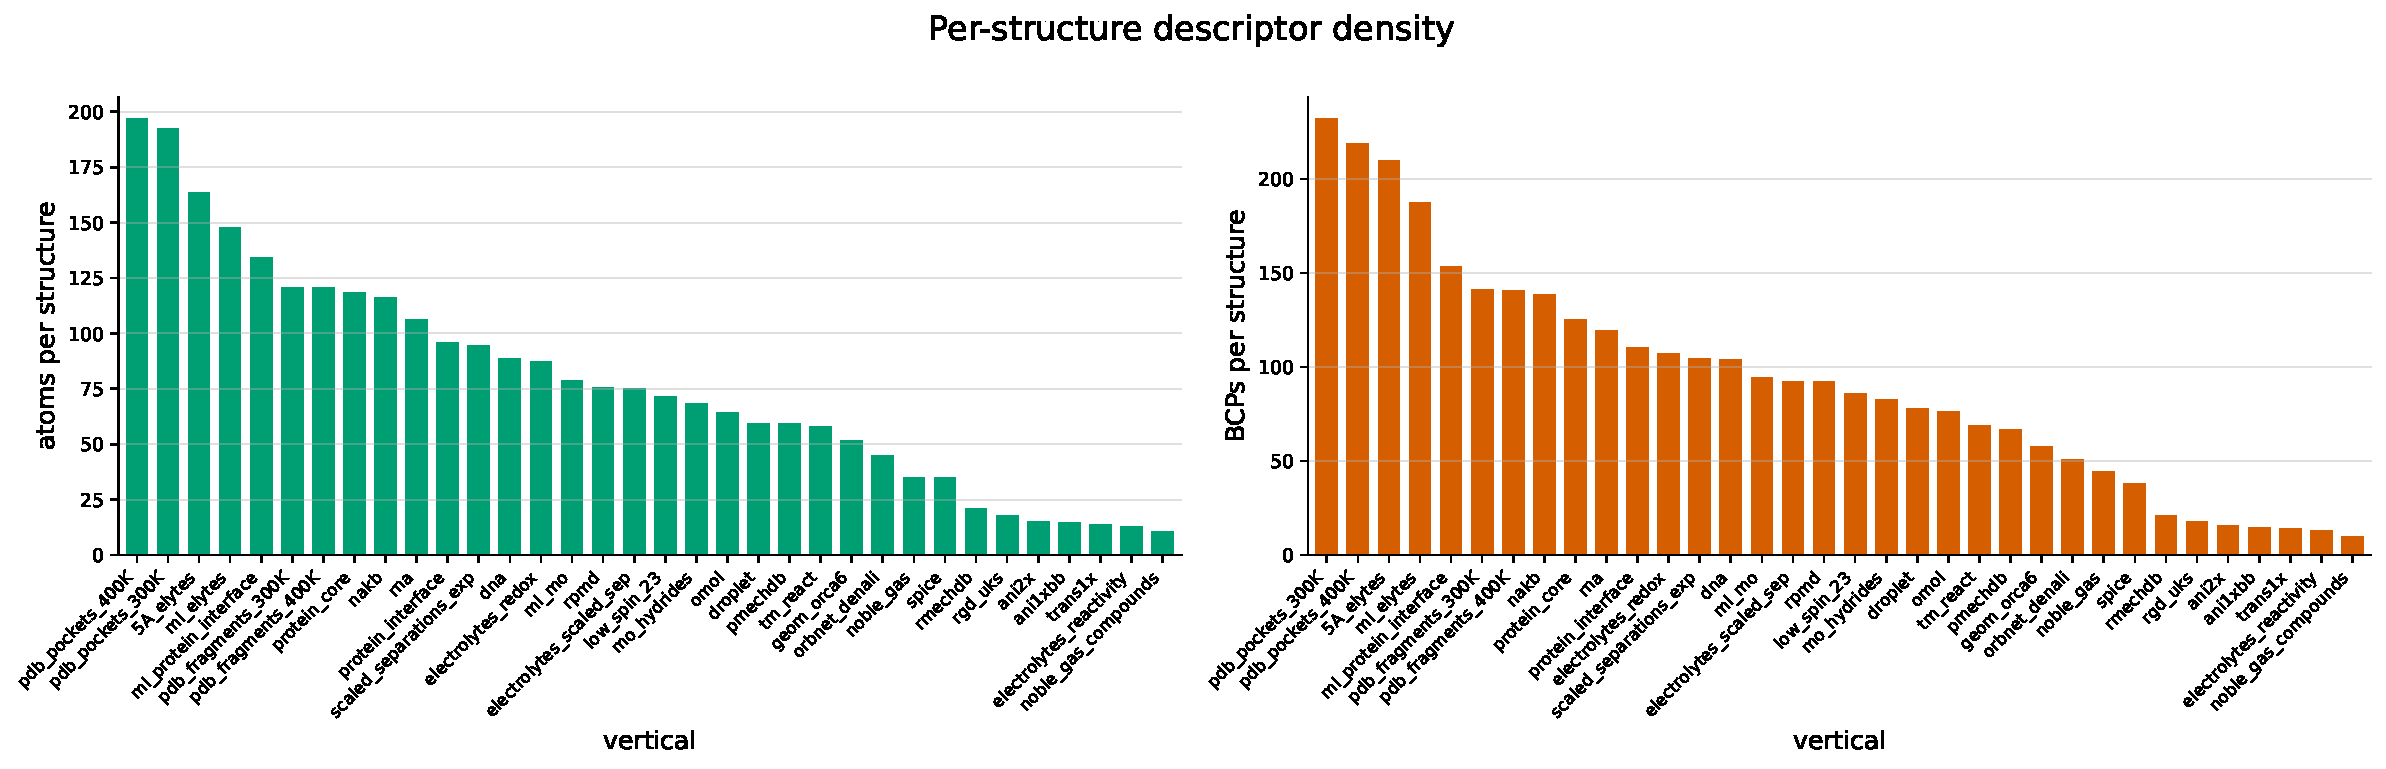
\includegraphics[width=\textwidth]{figures/census/descriptor_density.pdf}
\caption{Per-structure descriptor density across the 34 verticals.
Left: atoms per structure. Right: QTAIM bond critical points per
structure. Solvated-protein verticals (\texttt{pdb\_pockets\_300K},
\texttt{pdb\_pockets\_400K}, \texttt{protein\_core}) form the high-density
tail; \texttt{noble\_gas\_compounds} sits at the low end as the sparse
limit.}
\label{fig:descriptor_density_app}
\end{figure}

\begin{figure}[h]
\centering
\includegraphics[width=\textwidth]{figures/census/bond_scheme_breakdown_grouped.png}
\caption{Per-vertical bond-record counts shown as grouped bars rather than
stacked. The log-scale stack in Fig.~\ref{fig:bond_scheme_breakdown} compresses
the non-QTAIM schemes against the QTAIM BCP totals; the grouped view confirms
that Mayer, L\"owdin, and fuzzy bond records are within roughly an order of
magnitude of QTAIM BCP counts on every vertical, i.e. the four schemes have
comparable coverage rather than QTAIM dominating.}
\label{fig:bond_scheme_grouped_app}
\end{figure}


\subsection{Sharded Execution and LMDB Merge}
% Figure F4: sharding schematic.

LMDB is single-writer and exhibits lock contention under naive parallel writes, so
\texttt{json-to-lmdb} does not attempt to share a single output environment across workers.
Instead, each parallel job is given a shard index $i \in \{0, \dots, N-1\}$ and a total shard
count $N$, and partitions the input folder list by index modulo $N$. For the flat
\textit{root/category/subset/job} hierarchy this is a glob plus a modulo filter; for jagged
hierarchies such as OMol4M, where job folders sit at variable depth, the user supplies an
explicit \texttt{--folder\_list} file of absolute paths and the same modulo partitioning
applies to the line index. In both cases the LMDB key is
\texttt{relpath(folder, root\_dir).replace(os.sep, "\_\_")}, which is identical across every
descriptor family, so the per-family shards always share keys and joining is trivial.

Each shard writes into its own subdirectory as \texttt{shard\_\{i\}.lmdb}. When the last
shard finishes its work it drops a sentinel file (\texttt{shard\_N.done}); the merge step
waits on the full sentinel set and then concatenates per-family shards into a single
consolidated LMDB per family. The same shard/merge pattern is implemented at the converter
stage in \texttt{converter.py}, so graph construction can also be parallelized and joined
into one final per-vertical graph LMDB.


\section{LMDB Conversion Quality Audit}
\label{app:lmdb_audit}

Table~\ref{tab:lmdb_quality} reports raw failure counts per vertical from the
post-conversion audit (\texttt{lmdb\_status\_audit.py}).
\textit{QTAIM fail}: records where the \texttt{qtaim.lmdb} entry is empty,
malformed, or unpickleable.
\textit{ORCA fail}: same for \texttt{orca.lmdb} (includes SCF non-convergence
flagged at the parse stage).
\textit{Other fail}: failures across \texttt{structure}, \texttt{charge},
\texttt{bond}, \texttt{fuzzy}, and \texttt{other} LMDBs (all zero in this
release).
\textit{Max drop}: largest number of \texttt{structure.lmdb} keys absent from
any single descriptor LMDB; values $\leq 4$ across all verticals.

\begin{table}[h]
\centering
\caption{Per-vertical LMDB conversion-quality audit. Verticals with all
zeros across the four failure columns are shown as ``--''.}
\label{tab:lmdb_quality}
\begin{tabular}{lrrrrr}
\toprule
Vertical & $N$ & QTAIM fail & ORCA fail & Other fail & Max drop \\
\midrule
  \texttt{omol} & 1,429,192 & 17 & 896 & 0 & 1 \\
  \texttt{ani1xbb\_reparse} & 737,210 & 2 & 0 & 0 & 0 \\
  \texttt{ani2x} & 215,642 & -- & -- & -- & -- \\
  \texttt{trans1x} & 213,731 & -- & -- & -- & -- \\
  \texttt{geom\_orca6} & 199,805 & -- & -- & -- & -- \\
  \texttt{tm\_react} & 158,190 & 0 & 1 & 0 & 0 \\
  \texttt{pdb\_fragments\_300K} & 93,334 & 0 & 0 & 0 & 1 \\
  \texttt{pdb\_fragments\_400K} & 92,698 & -- & -- & -- & -- \\
  \texttt{ml\_mo} & 77,603 & 1 & 23 & 0 & 0 \\
  \texttt{rgd\_uks} & 75,316 & -- & -- & -- & -- \\
  \texttt{electrolytes\_reactivity} & 66,974 & 0 & 7 & 0 & 0 \\
  \texttt{ml\_protein\_interface} & 61,859 & 0 & 3 & 0 & 0 \\
  \texttt{scaled\_separations\_exp} & 53,219 & 2 & 37 & 0 & 0 \\
  \texttt{ml\_elytes} & 51,599 & 1 & 38 & 0 & 0 \\
  \texttt{orbnet\_denali} & 51,102 & -- & -- & -- & -- \\
  \texttt{pmechdb} & 49,832 & -- & -- & -- & -- \\
  \texttt{electrolytes\_redox} & 46,081 & 0 & 12 & 0 & 0 \\
  \texttt{protein\_interface} & 44,972 & 0 & 212 & 0 & 0 \\
  \texttt{spice} & 44,450 & 1 & 2 & 0 & 4 \\
  \texttt{protein\_core} & 35,406 & -- & -- & -- & -- \\
  \texttt{rna} & 34,745 & 0 & 311 & 0 & 0 \\
  \texttt{electrolytes\_scaled\_sep} & 30,769 & 0 & 1 & 0 & 0 \\
  \texttt{dna} & 24,647 & -- & -- & -- & -- \\
  \texttt{droplet} & 18,694 & -- & -- & -- & -- \\
  \texttt{rpmd} & 18,652 & 0 & 0 & 0 & 1 \\
  \texttt{pdb\_pockets\_300K} & 16,927 & 0 & 57 & 0 & 0 \\
  \texttt{5A\_elytes} & 14,202 & 0 & 2 & 0 & 2 \\
  \texttt{low\_spin\_23} & 12,939 & -- & -- & -- & -- \\
  \texttt{nakb} & 5,606 & -- & -- & -- & -- \\
  \texttt{mo\_hydrides} & 3,396 & -- & -- & -- & -- \\
  \texttt{pdb\_pockets\_400K} & 3,210 & 1 & 5 & 0 & 0 \\
  \texttt{rmechdb} & 2,803 & -- & -- & -- & -- \\
  \texttt{noble\_gas} & 1,915 & -- & -- & -- & -- \\
  \texttt{noble\_gas\_compounds} & 18 & -- & -- & -- & -- \\
\midrule
  \textbf{Total} & 3,986,738 & 25 & 1607 & 0 & 4 \\
\bottomrule
\end{tabular}
\end{table}

\vspace{1em}
Figure~\ref{fig:descriptor_coverage} shows per-method descriptor coverage
across all 34 verticals. Rows are descriptor methods grouped by family;
columns are verticals ordered by structure count (largest left).
Universal methods (Hirshfeld, ADCH, CM5, Becke charges; Fuzzy bond orders;
ORCA Mayer/L\"owdin/SCF/gradient/dipole) reach $\geq$99\% on every vertical.
QTAIM critical-point records achieve $\geq$99.9\% coverage.

\begin{figure}[h]
\centering
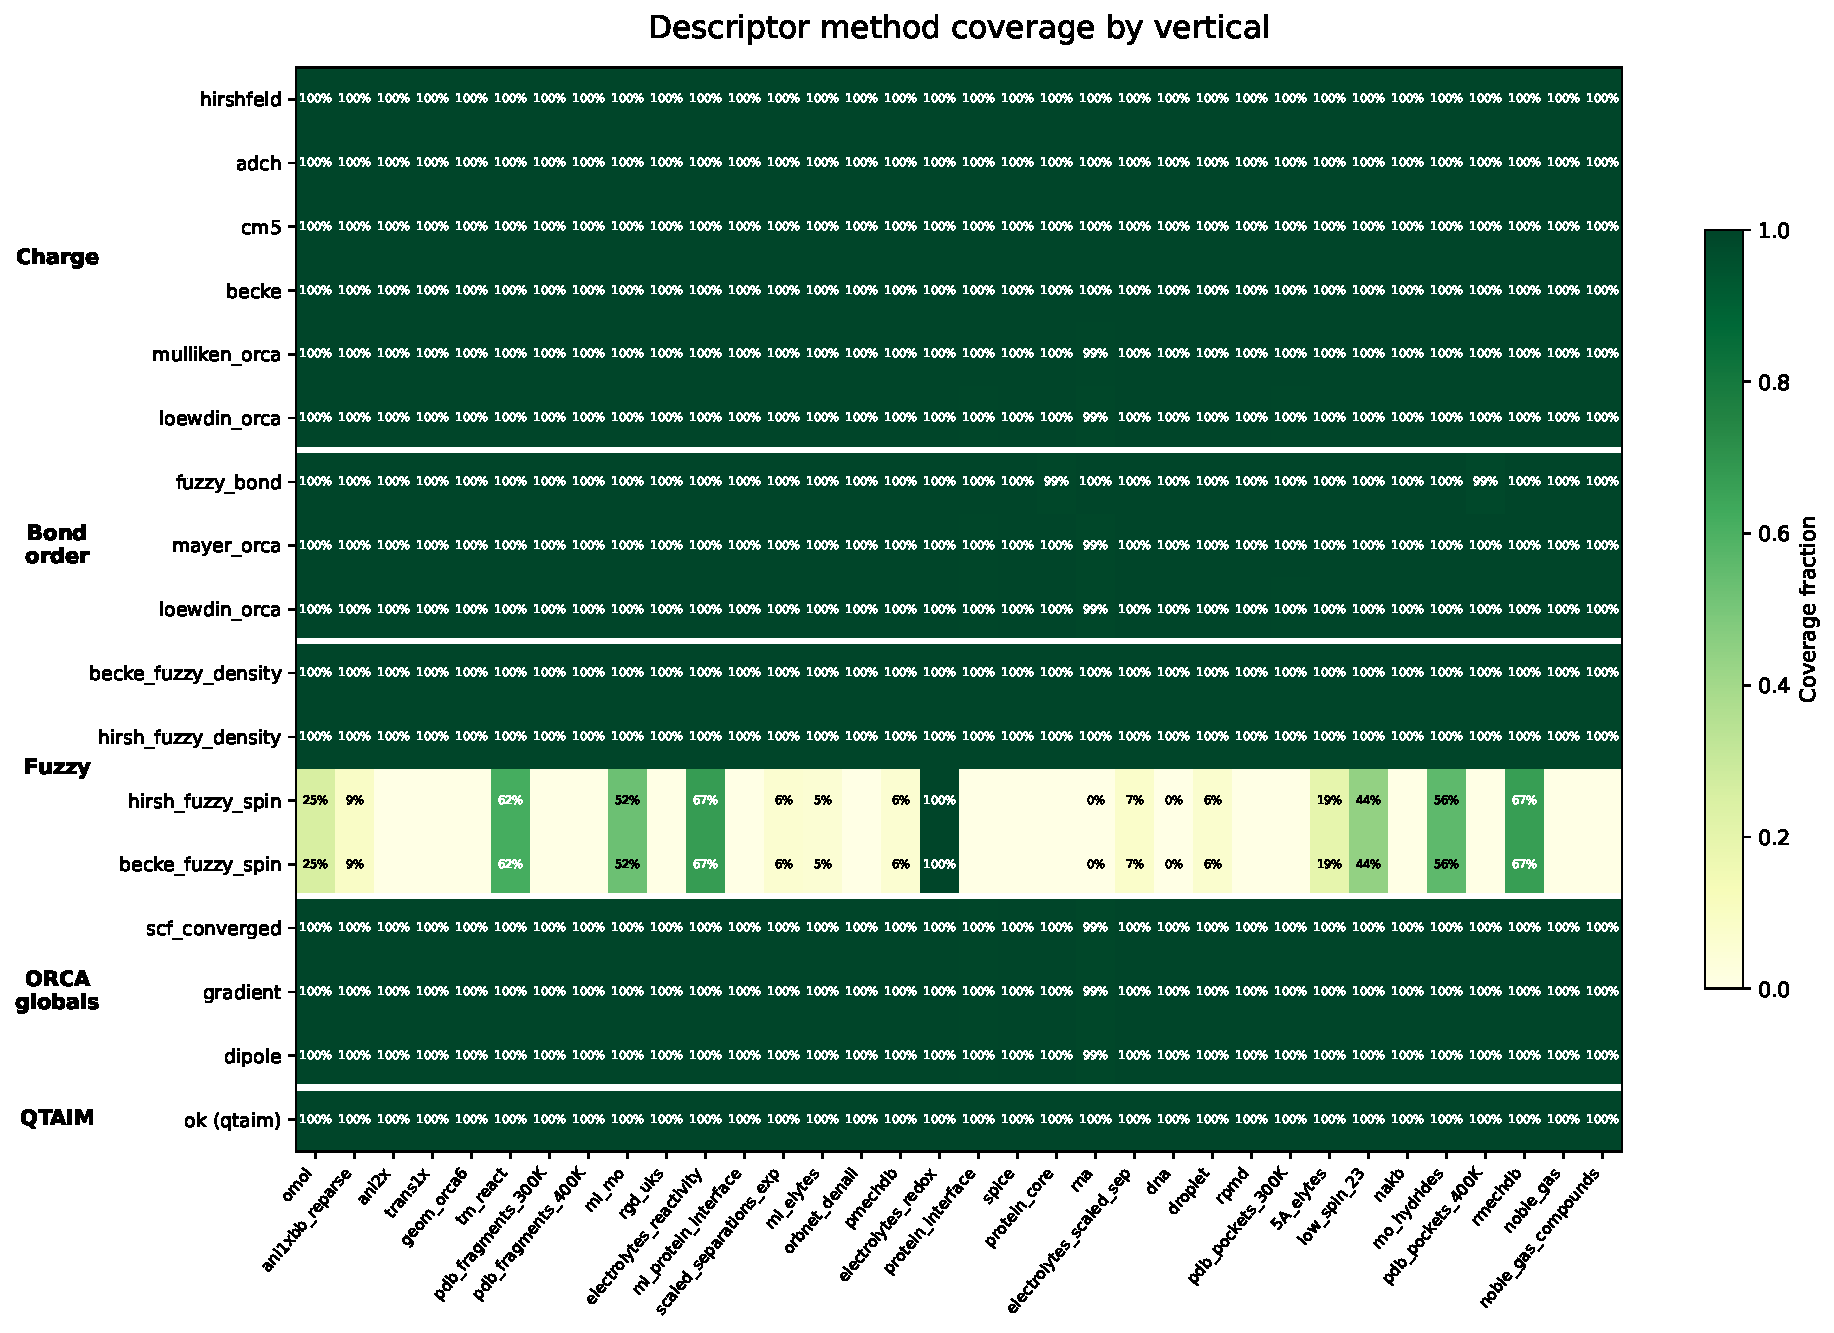
\includegraphics[width=\textwidth]{figures/dataset/dataset_coverage_heatmap.pdf}
\caption{Per-method descriptor coverage fraction across all 34 verticals.
Green = full coverage; white = absent. Vertical white lines separate
descriptor families. The single \texttt{ok (qtaim)} column reports
$\texttt{qtaim.lmdb}$ record validity.}
\label{fig:descriptor_coverage}
\end{figure}


\section{Charge-Scheme Cross-Correlations}
\label{app:charge_correlations}

We quantify pairwise agreement across the six partial-charge schemes
(Hirshfeld, CM5, ADCH, Becke, Mulliken, L\"{o}wdin) using two symmetric
metrics computed over all atom-level charge records in the corpus:
pairwise $R^2$ (coefficient of determination between scheme $a$ and scheme $b$
over all atoms) and mean absolute error (MAE, in electron units).
Figures~\ref{fig:charge_pearson_overall} and~\ref{fig:charge_mae_overall}
show the corpus-wide matrices; Figures~\ref{fig:charge_pearson_per_element_class}
and~\ref{fig:charge_pearson_tm} break these down by element class and by individual
transition metal; Figure~\ref{fig:charge_pearson_per_vertical} shows per-vertical matrices.

\begin{figure}[h]
\centering
\includegraphics[width=0.55\textwidth]{figures/charge/corpus_charge_pearson_overall.png}
\caption{Corpus-wide pairwise $R^2$ between charge schemes over all $\sim$218M atom
records. Hirshfeld--CM5 ($R^2=0.77$) and Hirshfeld--ADCH ($R^2=0.53$) show the
strongest cross-scheme agreement; Mulliken and L\"{o}wdin correlate weakly with
the stockholder-partitioned schemes ($R^2 \leq 0.30$).}
\label{fig:charge_pearson_overall}
\end{figure}

\begin{figure}[h]
\centering
\includegraphics[width=0.55\textwidth]{figures/charge/corpus_charge_mae.png}
\caption{Corpus-wide pairwise MAE (in $e$) between charge schemes.
Hirshfeld--CM5 (0.093~$e$) and Hirshfeld--ADCH (0.113~$e$) have the smallest
cross-scheme deviation. Mulliken diverges most ($\geq$0.37~$e$ versus
Hirshfeld/CM5/ADCH; 0.469~$e$ versus L\"{o}wdin), consistent with its
basis-set sensitivity at the def2-TZVPD level used throughout OMol25.}
\label{fig:charge_mae_overall}
\end{figure}

\begin{figure}[h]
\centering
\includegraphics[width=0.9\textwidth]{figures/charge/corpus_charge_pearson_per_element.png}
\caption{Pairwise $R^2$ stratified by element class: main-group, transition-metal,
lanthanide, and noble-gas subsets. Inter-scheme agreement tracks the corpus-wide
pattern within main-group chemistry; transition metals and lanthanides show reduced
Hirshfeld--ADCH agreement, reflecting the influence of $d$/$f$ polarization on
atomic-basin integration.}
\label{fig:charge_pearson_per_element_class}
\end{figure}

\begin{figure}[h]
\centering
\includegraphics[width=0.85\textwidth]{figures/charge/corpus_charge_pearson_transition_metals.png}
\caption{Pairwise $R^2$ broken down by individual transition-metal element
(30 panels, $n$ = atoms bearing that TM across all 34 verticals).
Each panel uses the same 6-scheme axis as Figure~\ref{fig:charge_pearson_overall}.
Variation across TMs is substantial: early 3$d$ metals (Sc, Ti, V) retain
moderate Hirshfeld--CM5 agreement ($R^2 \sim 0.4$--0.5) while late 4$d$/5$d$
metals (Pd, Pt, Au) drop to $R^2 < 0.3$, indicating that the connectivity
correction in CM5 diverges from the stockholder partition for electron-rich
coordination environments.}
\label{fig:charge_pearson_tm}
\end{figure}

\begin{figure}[h]
\centering
\includegraphics[width=0.85\textwidth]{figures/charge/per_vertical_charge_pearson.png}
\caption{Per-vertical pairwise $R^2$ across all 34 verticals (34 panels).
Organic-heavy verticals (\texttt{ani1xbb}, \texttt{spice}, \texttt{trans1x})
reproduce the high Hirshfeld--CM5 corpus agreement; TM-rich verticals
(\texttt{tm\_react}, \texttt{ml\_mo}, \texttt{mo\_hydrides}) show characteristically
lower cross-scheme $R^2$, particularly for Becke and L\"{o}wdin.
\texttt{noble\_gas} and \texttt{noble\_gas\_compounds} have near-zero off-diagonal
entries, as partial charges on noble-gas atoms are close to zero for all schemes.}
\label{fig:charge_pearson_per_vertical}
\end{figure}

\section{OMol-Descriptors-4M vs.\ tmQM+ Structural Overlap}
\label{app:umap_omol_vs_tmqmplus}

The main-text SOAP-UMAP comparison (Fig.~\ref{fig:umap_coverage}) uses a
6-element species basis (H, C, N, O, S, Cl) shared with the two organic
descriptor comparators (QM7-X, SchNet4AIM). That basis silently drops
transition-metal atoms during the SOAP fingerprint and therefore cannot
fairly place tmQM+ \citep{D5DD00220F} on the same map. We refit a separate
UMAP at a 32-element TM-inclusive species basis -- the 12 organic species
plus the first-row transition metals (Sc--Zn) and the 2nd/3rd-row TMs
(Mo, Ru, Rh, Pd, W, Re, Ir, Pt, Au, Hg) that exceed 1\% structure share
in either dataset -- with $r_{\mathrm{cut}}=5.0$~\AA, $n_{\max}=8$,
$l_{\max}=6$, dim$\,=\,$230{,}272. Per-source SOAP parquets total
$\sim$159k OMol-Descriptors-4M structures (drawn across all 33 verticals
that ship a \texttt{structure.lmdb}) and 12{,}147 tmQM+ structures from
the high-LOT split of the tmQM+ figshare deposit. Because pyNNDescent is
prohibitively slow at this dimensionality, dim reduction first projects
every SOAP vector to 256 components via a deterministic
GaussianRandomProjection (Johnson--Lindenstrauss; seed=42); UMAP fits on
the projected anchor sample and projects the remaining rows via
\texttt{reducer.transform}. We sample 50\% of the rest set per parquet
to cap wall time, leaving 81{,}945 OMol-Descriptors-4M points and 8{,}574
tmQM+ points on the canvas. The reproducibility script is
\texttt{notebooks/fit\_umap\_pca\_full.py} and the render is
\texttt{notebooks/render\_umap\_omol\_vs\_tmqmplus.py}.

\begin{figure}[h]
\centering
\includegraphics[width=\textwidth]{figures/umap/umap_omol_vs_tmqmplus_paper.pdf}
\caption{SOAP-UMAP embedding of OMol-Descriptors-4M (gray) against tmQM+
(orange) at the 32-element TM-inclusive SOAP basis. tmQM+ sits entirely
inside the TM-coordination region of OMol-Descriptors-4M (upper-central
cluster, UMAP-1 $\approx$ 5--14, UMAP-2 $\approx$ 9--15). The lower
gray-only territory (UMAP-2 $\approx$ 0--7) and the bottom-right tongue
(UMAP-2 $\approx$ -3, UMAP-1 $\approx$ 12) hold OMol's organic,
electrolyte, and protein-pocket chemistry that tmQM+ does not span. The
left-hand island (UMAP-1 $\approx$ -5) corresponds to the noble-gas and
noble-gas-compounds verticals.}
\label{fig:umap_omol_vs_tmqmplus}
\end{figure}

%\section{Extended Bond-Order Histograms}
%\label{app:bond_hists}

%\section{Additional Cross-Method Residual Plots}
%\label{app:residuals}



\section{Throughput and Parallel Scaling}
\label{app:throughput}

Here we report a local scaling experiment where we intent to show the concurrency performance
of Multiwfn on our routines. The local sweep is run on 16 copies of a moderately-sized structure drawn from
the dataset (from the droplet vertical here). It contains 36 atoms where we ran the three levels
of calculations in triplicate with Multiwfn 3.8. We sweep the number of concurrent job-folder
workers $\in \{1, 2, 4, 16\}$ at a fixed budget of cores (16) running to unearth how concurrency impacts wallclock.
The configurations are W16T1 (16 workers $\times$ 1 thread/job), W4T4 (4 workers $\times$ 4 threads/job), W2T8
(2 workers $\times$ 8 threads/job), and W1T16 (1 worker $\times$ 16 threads/job). Here we see that single-threaded
jobs yield the best performance with lower wallclock times across all three calculation levels. Thus, we
recommend users to prioritize more workers with fewer threads per job assuming that you do not run into memory bottlenecks
on larger systems with more memory-intensive routines.

\begin{figure}[h]
\centering
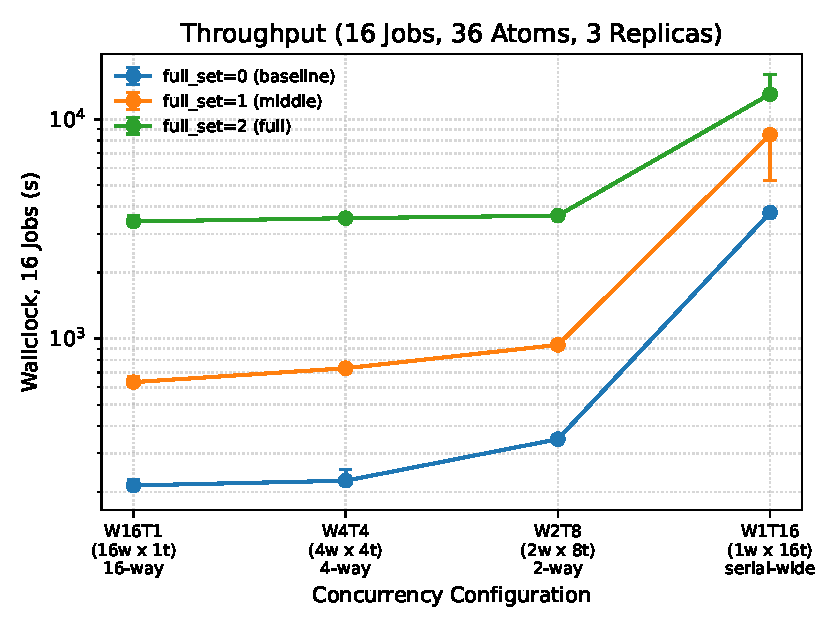
\includegraphics[width=0.75\textwidth]{figures/profiling_study/throughput_curves.pdf}
\caption{Multiwfn QTAIM post-processing wallclock as a function of intra-node concurrency
configuration. Each configuration processes 16 homogeneous copies of \texttt{droplet\_test}
(36 atoms, def2-TZVPD) under cascade-restart tiers. Configurations saturate a 16-thread
budget differently: W16T1 (16 workers $\times$ 1 thread), W4T4 (4 workers $\times$ 4 threads),
W2T8 (2 workers $\times$ 8 threads), W1T16 (1 worker $\times$ 16 threads). Each curve represents
a calculation tier (\texttt{full\_set} 0=baseline, 1=middle, 2=full). Tiers 1 and 2 use
\texttt{--restart} from the prior tier, so per-tier totals are cumulative phase wallclocks.
Markers show medians across 3 replicates with min/max whisker error bars. Y-axis is logarithmic
to visualize the ~75$\times$ range spanning W16T1 tier 0 (fastest) to W1T16 tier 2 (slowest).
Hardware: AMD 7950X (16c/32t). ORCA 6.0.1 (\texttt{shared\_openmpi416}) with system OpenMPI
4.1.2; Multiwfn 3.8 (Oct 2024 dev). ORCA SCF is precomputed; this measures post-processing only.}
\label{fig:throughput_scaling}
\end{figure}
